% !TeX root = ../main.tex

\chapter{Problemdiskussion}\label{chapter:dimensionwise_refinement}

	%References for chapters work like this. blblbla see \refChapter{chapter:background}.
			
	%\section{Program Structure}
	
		%For program code, use the following structure:
		
		%\begin{figure}[htbp]
			%\centering
			%\begin{tabular}{c}
			%\begin{lstlisting}[language=python]
			%	# enter your code here (# marks a comment in python)
			%	def (stuff as stuff):
			%		x = 1
			%	\end{lstlisting}
			%\end{tabular}
			%\caption{Caption Example}
			%\label{fig:code_integrator}
		%\end{figure}
		
	\section{Problembeschreibung}
		Da es viele verschiedene Umsetzungen der virtuellen und erweiterten Realität gibt, steht man als Entwickler eines Mixed-Reality Programms über Kurz oder Lang vor einigen Hindernissen. Eines davon ist die Platzierung der Benutzeroberfläche, da hierbei im Gegensatz zu gewöhnlichen Desktop-Anwendungen keine Bildschirmränder oder vergleichbare Begrenzungen vorhanden sind.
		Zudem existiert keine konkrete Vorgabe wie die Benutzeroberfläche in der dreidimensionalen Welt platziert werden sollte. In bestehenden Programmen wird diese aber oft an Controllern platziert, wessen Position durch ein Ortungssystem erfasst wird. Eine Alternative bildet die Platzierung der Oberfläche rings um den Nutzer in Form eines Zylinders oder einer Kugel.
		Besondere Schwierigkeiten entstehen aber noch zusätzlich, wenn man das Programm auf verschiedenen Geräten nutzen möchte. So werden zum Beispiel bei vielen Varianten der erweiterten Realität die Handpositionen nie oder zumindest nicht kontinuierlich verfolgt und ermöglichen somit kein konstantes Anzeigen von virtuellen Elementen an diesen Stellen. Sie können daher schlecht als Ankerpositionen für die Benutzeroberfläche verwendet werden.
		Andere Geräte stellen durch die Positionserfassung der Controller und der VR- oder AR-Brille die Kopf- und Handpositionen zu jeder Zeit zur Verfügung. Das Wegfallen von Controllern durch niedrigen Akkustand oder andere Umstände erzeugt dabei allerdings ein ähnliches Problem wie bei den Varianten ohne solche Controller.
		Da die Positionierung der Benutzeroberfläche an den Handpositionen deren Elemente näher zum Nutzer bringt und eine intuitive Art zum Verstecken von Informationen bietet, sollten diese auch genutzt werden, solange diese Positionen vorhanden sind. Für den Fall ihrer Abwesenheit ist es dann allerdings nötig eine Rückfallmöglichkeit bereitzustellen, damit keine Elemente der Benutzeroberfläche verloren gehen und mit ihnen deren Funktion und Information. Diese Verluste könnten sonst eine produktive Nutzung erschweren oder sie sogar gänzlich verhindern.
		
	\section{Ansatz}
		Um die Verwendung von allen Elementen der Benutzeroberfläche auch beim Verlust einer oder mehrerer möglicher Ankerpositionen zu gewährleisten, wurden in dieser Arbeit mehrere Möglichkeiten erarbeitet, um eine Umverteilung der enthaltenen Informationen von einem nicht verwendeten Anker auf einen oder mehrere aktive Anker durchführen zu können.
		Dafür wird betrachtet wie wichtig die einzelnen Inhalte sind, welche aktiven Ankerpositionen zur Verfügung stehen und was für eine Rückfallart bei der Verschiebung verwendet werden soll. Letztere entscheidet darüber wie der Rückfall aufgefangen wird.
		Die Neuplatzierung der umverteilten Bausteine übernimmt jeweils der neue Anker.
		
		\subsection{Umsetzung der Prioritätsstufen}
			Um herauszufinden wie wichtig ein Element ungefähr ist, werden erst klare Klassen benötigt, welche unterschiedliche Prioritäten darstellen. Diese entscheiden darüber wie und wo eine Information dargestellt wird und ebenso wohin sie, im Falle des Verlusts des zugehörigen Ankers, verschoben wird.
			Als Vorbild für das in dieser Arbeit verwendete Modell dienen die in \refChapter{chapter:prio} genannten Kategorien.
			%- vorbild S.H.I.T.
			%- wichtig für Verarbeitung bei Fallback
			Es gliedert sich in die vier Stufen \term{high}, \term{medium}, \term{low} und \term{none}. Diese werden abhängig von dem aktuellen Kontext und dem Typ des zugehörigen Ankerposition wie folgt umgesetzt:
			%- High/Medium/Low/None
			%Zudem wurde es abhängig vom aktuellen Kontext und dem Typ der Ankerposition gemacht.
			%- Kontextabhängigkeit
			
			An einer Handposition werden Informationen mit den Prioritäten \term{high} und \term{medium} gleich behandelt. Sie sind, im Gegensatz zu den Prioritäten \term{low} und \term{none}, nicht manuell ausschaltbar, aber können dennoch durch das Bewegen der Hand aus dem Sichtfeld entfernt werden. Beim Wegfall der Handposition werden alle Elemente der Stufen \term{high}, \term{medium} und \term{low} einem anderen Anker zugewiesen. Ein Inhalt aus der Kategorie \term{none} wird nur an andere Hand-Anker weitergeleitet, nicht jedoch an Kopf-Anker.
			
			%Hand:
			%-Hoch Immer angezeigt
			%-Medium Immer angezeigt
			%-Low Zuschaltbar
			%-None Zuschaltbar 
			
			An einem Kopf-Anker findet kein Zusammenschluss von diesen vier Stufen statt. Dort wird ein Exemplar der Kategorie \term{high} immer im Sichtfeld des Nutzers angezeigt. \term{medium} und \term{low} werden wie bei einem Hand-Anker behandelt und ein Objekt mit Priorität \term{none} sollte es dort nicht geben.
			
			%Kopf:
			%-Hoch: immer angezeigt, immer sichtbar
			%-Medium immer angezeigt
			%-Low Zuschaltbar
			%-None Fällt weg
			
		\subsection{Rückfallarten}\label{chapter:fallback}
			Für die Umverteilung der Ankerinhalte wurden drei Methoden entworfen, welche diese Aufgabe auf verschiedene Art verwirklichen. Dabei wurde jeweils unterschiedlich viel Wert auf individueller Platzierung, Automatisierung und Nutzbarkeit gelegt.
			
			%- Über ID
			Eine Variante, welche manuelles Platzieren erlaubt, ist die Verschiebung über eine Identifikationsnummer. Dabei werden, gegebenenfalls veränderte, Kopien des zu verschiebenden Inhalts bereits vorher auf den Rückfall-Ankern platziert. Beim Wegfallen des Ankers wird dann lediglich auf diesen Ankern nach einem Element mit der gleichen Identifikationsnummer gesucht und dieses aktiviert. Der Nachteil dieser Option ist, dass für jedes Element manuell alle Ausweichpositionen definiert werden müssen. Dies bietet aber auch den Vorteil, dass eine Information nie an eine ungewollte Stelle rückt, sondern genau so angezeigt wird, wie es durch den Ersteller vorgegeben wurde. Es lässt also ein individuelles Abfangen zu.
			
			
			%- Über Container
			Eine andere Option, welche ein automatisiertes geordnetes Platzieren umsetzt, benötigt eine Art Container für Inhalte. Ein Beispiel für einen solchen Container sind die Anker selbst, da sie ebenso Elemente enthalten. Allerdings ordnen diese von sich aus keine neuen Informationen auf bestimmte Weise neben den Bestehenden an, sondern übergeben diese Aufgabe an andere Container, welche in ihnen enthalten sind. Die Art und Weise wie ein Container neue Inhalte handhabt muss manuell festgelegt werden und wird dann zur Laufzeit automatisiert ausgeführt. Somit fällt, im Vergleich zu dem Rückfall mit ID, der Aufwand des manuellen Platzierens weg. Dafür muss hingegen eine Logik für den Container entworfen werden und die Umsetzung wird weniger individuell, wodurch es zu ungewollten Anordnungen von Elementen kommen kann.
			
			
			%- Innerhalb eines Containers
			Zuletzt gibt es noch eine Art der Verschiebung, bei der die betroffenen Elemente innerhalb ihres Behälters bleiben und dieser dann mitsamt seinem Inhalt als ein Objekt verschoben wird. Dabei muss der Zielanker auf eine, in \refChapter{chapter:expand} beschriebene, Weise erweitert werden, da dem Anker die genaue Lage des Inhalts nicht bekannt ist. Diese Variante ist auf eine Nutzeroberfläche im Stil eines Gitters mit rechteckigen Elementen ausgelegt. Eine Verwendung mit anderen Stilen oder in Verbindung mit weiteren Rückfallarten kann Lücken zwischen den Elementen erzeugen. Sie erfordert dazu aber keine weitere Arbeit seitens des Erstellers.
			%- Wichtigkeit entscheidet über nutzbare Anker
			
			
			Bei allen Varianten wird geprüft ob die Priorität des verschobenen Objekts höher oder gleich wie die Mindestpriorität des Zielankers ist, um jederzeit möglichst nur die benötigte Information anzuzeigen und unwichtige Inhalte gegebenenfalls zu verbergen. Falls die Priorität nicht zu dem Anker passen sollte, wird das Verfahren auf einem anderen Anker weitergeführt, solange noch ein weiterer zur Verfügung steht.
			
		\subsection{Erweiterung}\label{chapter:expand}
			Wie bereits in \refChapter{chapter:fallback} erwähnt, kann es vorkommen, dass ein Anker durch das Hinzufügen von Informationen gegebenenfalls erweitert werden muss, um die zusätzlichen Elemente platzieren zu können. Dazu wurden zwei Varianten erarbeitet. Welche davon verwendet werden soll, muss in jedem Anker manuell angegeben werden.
			
			%- Directional
			Die erste Art erweitert den Bereich, in dem der Inhalt platziert werden kann, in eine vorgegebene Richtung. Daraufhin werden darin neuer und alter Inhalt untereinander beziehungsweise nebeneinander platziert. Somit wird ein Überschneiden von Elementen verhindert.
			

			Die andere Variante erzeugt eine Schaltfläche, mit deren Hilfe zwischen der Anzeige von den alten und den neuen Informationen gewechselt werden kann. Somit wird durch neuen Inhalt nicht mehr Platz eingenommen. Allerdings kann man dadurch die verschiedenen Informationen nicht alle gleichzeitig sehen.
			
	\section{Umsetzung}
		Um diesen Ansatz umzusetzen wurden im Programm \term{Visual Studio 2015} mit der Programmiersprache C\# die Klassen \term{UIAnchor}, \term{AnchoredUI}, \term{AnchorManager} und das Interface \term{UIContainer} erstellt. Sie stellen die Funktionen zur Manipulation der Benutzeroberfläche zur Verfügung. Deren Funktionsweise wird in den nachfolgenden Abschnitten beschrieben.
		
		
		\subsection{AnchoredUI}
			Die einzelnen Elemente der Benutzeroberfläche werden durch Instanzen dieser Klasse repräsentiert. Sie beinhaltet Informationen für deren Verschiebung auf andere Anker. Dazu zählen ihre Priorität und die Rückfall-Variante. Bei dem Verlust ihres Ankers wird in der \term{AnchoredUI}-Instanz eine Funktion aufgerufen, welche über die Art ihres Neuplatzierens bestimmt und dieses daraufhin startet.
			%- Stellt Element dar
			%- Beinhaltet Informationen für die Fallback Umsetzung
		
		\subsection{UIContainer}
			
			Dieses Interface dient als Vorlage für Behälter von Instanzen der Klasse \term{AnchoredUI}. \linebreak Diese Container enthalten eine Logik zum systematischen Platzieren von neuen\linebreak Elementen innerhalb des bereits vorhandenen Inhalts und dienen dazu, eine automatische Verschiebung und geordnete Neuplatzierung von Ankerinhalten individueller gestalten zu können.
			%- enthält Elemente
			%- ermöglicht strukturierte Platzierung von dynamischem Inhalt
			
		\subsection{UIAnchor}
			Die Klasse \term{UIAnchor} stellt einen Anker für Bestandteile der Benutzeroberfläche dar. Sie beinhaltet unter anderem die Attribute \term{style} und \term{type}, welche angeben, inwiefern der Inhalt des Ankers manipuliert werden soll. Der Wert \term{type} steht dafür, ob der Anker am Kopf, der rechten oder der linken Hand angebracht ist. Die Variable \term{style} definiert, ob enthaltene Elemente in einer Ebene (Wert: Rectangle) oder auf einem Zylinder (Wert: Cylinder), mit dem angegebenen Radius \term{distance}, um den Anker herum angeordnet werden sollen. Darüber wird dann gemeinsam mit der Priorität des Ankers die Positionierung der enthaltenen \term{AnchoredUI}-Instanzen durchgeführt.
			Als Vorbild für die Umsetzung des Stils \term{Cylinder} an der Kopfposition fungierte eine Abwandlung des Prinzips, das unter Anderem in Planetarien genutzt wird (siehe \refFigure{fig:cylinder_mapping}).
			
			Für einen Kopf-Anker mit dem Stil \term{Rectangle} und der Priorität \term{medium} wurde das Standardmenü der Hololens (siehe \refFigure{fig:hololensMain}) als Vorlage genommen. Das Menü wird in diesem Fall also nicht immer an der gleichen Stelle des Sichtfelds angezeigt, sondern bleibt so lange unbewegt, bis es aus dem Blickfeld verschwinden würde. Dann bewegt es sich wieder in die Sicht des Nutzers. Somit blockiert der Inhalt des Menüs nicht so sehr das Blickfeld, obwohl er durchgehend angezeigt wird.
			%- Cylinder (Beispiel Bild bereits verwendet - Referenz)
			%- Rectangle bei Fehlenden Controllern high or medium prio
			%- Umsetzungen abhängig von Prio und Position
			%- Vorbild Rectangle Hololens
			\begin{figure}[htbp]
				\centering
				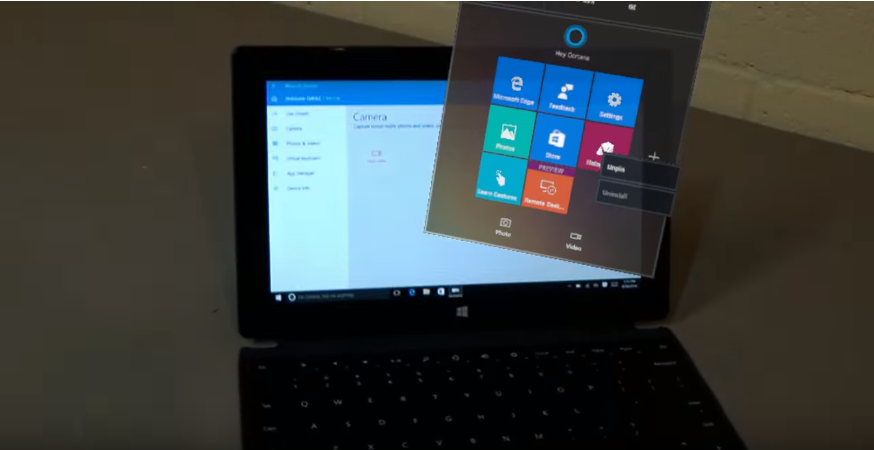
\includegraphics[width=0.75\textwidth]{figures/HololensMain.png}
				\caption{Menü der Hololens \takenFrom{hololens}.}
				\label{fig:hololensMain}
			\end{figure}
			%- Cylinder Abwandlung von Planetarium und Ähnlichem
			
			Außerdem hat er noch vier Attribute, welche seine Bindung zum zugehörigen Ankerobjekt darstellen. Eins gibt die relative Position des Ankermittelpunkts zur Mitte des Ankerobjekts an. Ein weiteres steht für die relative Rotation zu diesem Objekt. Die anderen beiden Variablen legen fest, ob und wie sich der Anker mit dem Ankerobjekt rotiert.
			%- Rotation/Translation zu Ankerposition
			%- Erweiterungsart
			%- minprio
			%- statictoObj
			%- rotates
			%- stellt Anker dar
			Zudem besitzt die Klasse eine optionale Referenz auf eine weitere Ankerinstanz, welche im Nachfolgenden \term{Kindanker} genannt wird. Diese sollte im Normalfall eine niedrigere Mindestpriorität besitzen und vom gleichen Typ sein, denn sie dient als weitere Möglichkeit für die Platzierung von Inhalten, falls diese in dem Anker mit höherer Mindestpriorität keinen Platz finden. Außerdem wird durch die Kindanker das Platzieren mehrerer Anker an einem einzelnen Objekt ermöglicht. Bei der Deaktivierung eines Ankers wird ebenso dessen Kindanker deaktiviert.
			%- gibt Anweisungen an Kinderanker weiter
			%- Manipuliert Elemente abhängig von Ankertyp
			%- Setzt Fallback um
			Beim Nichtvorhandensein des Ankerobjekts, an der ein Anker platziert werden sollte, sucht dieser über die statische Klasse \term{AnchorManager} nach einem alternativen Ort, um seine Informationen weiterhin anzeigen zu können.
			Falls kein Anker dafür gefunden wurde, wird die Information verworfen und eine Warnmeldung angezeigt. Ansonsten wird versucht diesem den Inhalt zu übergeben. Der Zielanker berechnet dann mittels dessen Priorität, ob er die Informationen bei sich platziert oder sie an einen Kindanker weiterleitet.
		
		\subsection{AnchorManager}
			Die statische Klasse \term{AnchorManager} wird beim Start der Anwendung über die Verfügbarkeit von Ankerobjekten informiert und übermittelt diese Informationen an das zugehörigen \term{UIAnchor}-Objekt. Sie startet damit auch das Wegfallen der Anker, falls deren Ankerobjekt nicht vorhanden sein sollte. Die Anker vermitteln die Informationen weiter an deren Kindanker und fragen im gegebenen Fall beim \term{AnchorManager} eine Ausweichoption ab. Bei der Auswahl einer Option werden Handanker in dieser Umsetzung immer bevorzugt.
			%- Regelt das Wegfallen von Ankern
			%- Weist FBAnker zu
			
	\section{Evaluierung}
		%- Studie
		%- 13 Teilnehmer
		Um die beschriebene Umsetzung zu evaluieren wurde eine Nutzerstudie durchgeführt, an der dreizehn Freiwillige im Alter zwischen 16 und 26 Jahren teilnahmen. Der Fragebogen zu dieser Studie wurde mit dem Programm LimeSurvey erstellt und befindet sich im Anhang dieser Arbeit (siehe ...)\todo{Referenz}. Dieses Kapitel beschreibt deren Aufbau und Ablauf.
	
		\subsection{Studienablauf}
			%- 4 Szenarien
			In der Studie mussten die Probanden in vier verschiedenen Szenarien jeweils eine Reihe von Aufgaben durchführen. Die Reihenfolge der vier Abschnitte wurde dabei jedes Mal variiert und war für jeden Teilnehmer unterschiedlich, um einen Einfluss der Bearbeitungsreihenfolge auf das Gesamtergebnis möglichst gering zu halten. Die Aufgabenstellung blieb in allen Szenarien die Gleiche.
			
			
						
			Zu Anfang sollten die Tester ein paar einleitende Fragen beantworten, dann führten sie die Aufgaben ein erstes Mal in einem der Szenarien durch und beantworteten danach Fragen zu diesem Testfall und einzelnen Elementen darin. 
			Dies beinhaltete zwei Fragen nach der gefühlten Schwierigkeit der Aufgabe innerhalb des Testfalls. Einmal sollten sie angeben ob sie gefühlt viel Zeit für die Aufgabe gebraucht haben, beim zweiten Mal mussten sie deren Schwierigkeit auf einer Skala von eins bis fünf bewerten, wobei eins für sehr leicht und fünf für sehr schwierig steht. Zusätzlich sollten sie angeben, ob sie die Positionierung der Benutzeroberfläche übersichtlich oder willkürlich fanden.
			
			
			Danach folgten jeweils drei Fragen zu sieben Elementen der Benutzeroberfläche aus der Testszene. Bei diesen konnten sie jeweils aus einer gegebenen Liste auswählen, ob und warum sie nach dem Element suchen mussten, es anstrengen anzusehen fanden oder es störend fanden. Eine nicht gelistete Antwort konnte ebenfalls angegeben werden.
			%- störend - anstrengend anzusehen - nicht findbar
			%- Aufzählung der Fragen
			
			Die zu bewertenden Elemente wurden so ausgewählt, dass jeweils mindestens zwei Beispiele aus den Prioritätsklassen \term{high}, \term{medium}, \term{low} und zwei kontextabhängige Exemplare bewertet wurden.
			%- Wie wurden zu bewertende Elemente ausgewählt?
			Die Auswahl dieser Elemente war ebenfalls in jedem Szenario gleich.
			
			Dies wurde viermal wiederholt. Zum Abschluss sollten sie noch angeben, wie schwierig sie die Aufgabenstellung und die Steuerung unabhängig von den Szenarien fanden und als wie wichtig sie die ausgewählten Elemente auf einer Skala von eins bis fünf einordnen würden. Die genauen Definitionen der verschiedenen Stufen wird in \refChapter{chapter:resultsPrio} beschrieben.
		
		\subsection{Szenario-Beschreibung}\label{chapter:szenario}
			In jedem der Testfälle hatten die Tester die Aufgabe mit einem offen sichtbaren Gegenstand zu interagieren. Dazu musste der \term{Cursor} auf diesen ausgerichtet werden. Der \term{Cursor} ist in der Mitte des Sichtfeldes platziert und bewegt sich beim Drehen und Neigen des Kopfes mit. Man wählt also im Groben ein Objekt aus indem man darauf schaut.
			Nach dem Interagieren mit dem Gegenstand öffnet sich ein verborgenes Menü, dessen Inhalt zylinderförmig um die Position des Nutzers aufgereiht ist. Dieses heißt im Folgenden \term{Handelsfenster}. Es beinhaltet zwölf Elemente mit je einem farbigen Würfel und einer Preisangabe, welche alle ausgewählt werden können.
			
			Als nächstes sollten die Tester herausfinden, wie viel Geld ihnen zur Verfügung steht und dann einen Würfel auswählen, dessen Preis die verfügbare Geldmenge nicht überschreitet. Diese Menge wird im Infofeld \term{Vermögen} angezeigt, welches nur bei geöffnetem Handelsfenster verfügbar ist.
			Daraufhin wird der ausgewählte Würfel gekauft und in das Feld \term{Ausgewähltes Objekt} verschoben, welches zu jeder Zeit angezeigt wird. Es informiert darüber, ob etwas gerade ausgewählt ist und um was es sich dabei handelt.
			
			Die letzten drei Schritte beinhalten das Legen des gekauften Würfels in eines der \term{Inventar}-Felder, das erneute Auswählen des Würfels und das Ablegen in ein Feld der \term{Ausrüstung}. Sowohl das \term{Inventar} als auch die \term{Ausrüstung} können manuell ein- und ausgeblendet werden. Wie dies funktioniert und wie die beiden Elemente erkannt werden können wurde den Teilnehmern vor dem Ausführen der Aufgabe erklärt.
			Danach gilt die Aufgabe als abgeschlossen.
			
			Die vier Szenarien unterscheiden sich nur in der Platzierung der genannten Elemente der Nutzeroberfläche. Sie simulieren jeweils das Vorhanden- oder Nichtvorhandensein der beiden realen Handpositionen im virtuellen Raum. \todo{Referenz auf Bilder im Anhang}
			
			
			In der Simulation von zwei Handpositionen werden die genannten UI-Elemente auf beide Hände verteilt. An der linken Seite befindet sich das \term{Inventar}, welches manuell verborgen und wieder sichtbar gemacht werden kann. Außerdem ist das \term{Vermögen} dort platziert, das nur bei geöffnetem Handelsfenster angezeigt wird. Auf der rechten Seite ist das \term{Ausgewählte Objekt} zu sehen und daneben die \term{Ausrüstung}, welche wie das \term{Inventar} aus- und eingeklappt werden kann.
			
			Die beiden Fälle mit nur einer Hand wurden so gelöst, dass die Oberflächen der einen Hand auf die andere übertragen wurde. Dabei unterschieden sich die Fälle darin, dass jeweils andere Erweiterungsarten (siehe \refChapter{chapter:expand}) verwendet wurden. Auf der rechten Seite war dies die Umsetzung mit der Schaltfläche.
			
			Bei der vierten Version mussten die Nutzer ohne Hände auskommen. \term{Inventar} und \term{Ausrüstung} waren dafür ähnlich zum \term{Handelsfenster} auf einer Zylinderoberfläche um den Nutzer herum angeordnet und konnten wie in allen anderen Fällen ein- und ausgeblendet werden. Das \term{Ausgewählte Objekt} und das \term{Vermögen} waren nach dem Vorbild des Standardmenüs der Hololens (siehe \refFigure{fig:hololensMain}) im Blickfeld des Testers befestigt. 
			
			%\todo{Beschreiben}
			%- Szenenbeschreibung
			%- verwendete UI Elemente
			%- Unterschiedliche Fälle
		